\chapter{Introduction}

VisuaLearn AI is a web-based learning platform built to help students study topics that are difficult to understand from plain text alone. The system combines conversational explanation, visual learning resources, simulations, quizzes, flashcards, document support, and saved learning history. It was developed as a full-stack application using a React frontend, an Express backend, Supabase for authentication and persistence, and large language model support through backend services.

\section[Background]{\textbf{Background}}

Online learning has become a regular part of student work. Students now use recorded classes, search engines, discussion forums, chatbots, and course platforms while preparing for assignments and examinations. These tools increase access to information, but they do not always provide the kind of support needed when a learner is confused. A short answer may define a term, but the same learner may also need a diagram, a worked example, a quiz, or a simulation before the idea becomes clear.

Studies on online and blended learning report that engagement remains a concern even when digital access is available \cite{Martin2018,Instructure2023}. Multimedia learning research also shows that combining words and visuals can improve understanding when both are presented in a coordinated manner \cite{Mayer2009}. Simulation-based learning has been shown to support procedural and complex skill development in higher education \cite{Chernikova2020}. These findings support the need for systems that do more than return text responses.

Many technical subjects require learners to move between different representations. In data structures, a student may know the definition of a queue but still struggle to follow how values enter and leave it. In sorting algorithms, the comparison and swap steps are easier to understand when the intermediate states are visible. Similar problems occur in recursion, graph traversal, memory allocation, CPU scheduling, and machine learning. VisuaLearn AI addresses this type of learning need by placing explanation, practice, visualization, simulation, and revision material in the same learning workspace.

\section[Literature Review]{\textbf{Literature Review}}

The project is based on ideas from multimedia learning, cognitive load theory, intelligent tutoring systems, adaptive learning, and AI-assisted education. Mayer's multimedia learning theory explains that learners benefit when verbal and visual information are connected meaningfully \cite{Mayer2009}. Sweller's cognitive load theory shows that learning is affected by the mental effort required to process new material \cite{Sweller1988}. These ideas support the use of concise explanations, diagrams, simulations, and gradual learning steps.

Bloom's work on one-to-one tutoring showed the value of individualized instruction \cite{Bloom1984}. Later studies on intelligent tutoring systems found that software tutors can improve learning when they track learner progress and provide timely feedback \cite{VanLehn2011,Ma2014}. Recent work on large language models in education shows that such models can generate natural language explanations, but it also warns about hallucination, weak feedback quality, and the need for careful educational design \cite{Kasneci2023}.

Existing learning systems often support one task well, such as answering questions, showing videos, giving quizzes, or managing course material. The gap addressed in this project is the lack of a single workflow that connects conversation, visual explanation, generated revision resources, document-aware learning, simulation, feedback, and history. VisuaLearn AI was developed to study how these parts can be organized into one application.

\section[Motivation]{\textbf{Motivation}}

The motivation for the project came from common student difficulties observed in technical learning. Static notes are useful for revision, but they are often insufficient when the topic has movement, order, state changes, or multiple interacting parts. Learners then search separately for diagrams, animations, examples, and practice questions. This breaks concentration and makes revision less organized.

For example, a student learning bubble sort may remember that adjacent values are compared, but may not see why the largest value reaches the end after one pass. A student learning recursion may understand the code line by line but fail to visualize the call stack. A student learning breadth-first search may know that a queue is used, but may not follow how the queue changes during traversal. These examples show why a learning platform should support both explanation and visual inspection.

The project is also motivated by differences between learners. A beginner may need an analogy and a simple example. A more prepared learner may need a compact explanation, code walkthrough, or quiz. A learner revising before a test may prefer flashcards, while a learner facing a misconception may need a slower step-by-step explanation. VisuaLearn AI records profile information and interaction signals so that later responses can be adjusted to the learner's context.

\section[Problem statement]{\textbf{Problem statement}}

Most digital learning tools provide isolated support for explanation, practice, visualization, or revision. They do not normally combine adaptive explanations, visual simulations, document context, generated revision artifacts, feedback, and persistent learning history in one place. This creates a fragmented learning experience and reduces continuity between asking a question, understanding the answer, practising the concept, and revising it later.

The problem addressed in this project is to design and implement a web-based AI learning platform that provides personalized, interactive, and persistent learning support. The platform must support normal conversation, structured learning resources, visual and simulation-based explanation, learner profiles, document-assisted responses, and feedback-based adaptation.

\section[Objectives]{\textbf{Objectives}}

The objectives of the project are:
\begin{enumerate}[leftmargin=1.2cm]
\item To design a full-stack agentic AI learning platform with authenticated users, persistent conversations, learning profiles, and adaptive tutoring support.
\item To implement an agent-based learning pipeline for streamed explanations, visual widgets, learning plans, document-based learning, simulations, 3D visualizations, video-oriented learning support, and optional voice interaction.
\item To provide a feedback and personalization mechanism that uses profile data, behavior, persona, and learning state to improve the relevance of future explanations.
\item To evaluate the usability and learning support of the system through participant testing, feedback analysis, and interaction observations.
\end{enumerate}

\section[Scope of Project]{\textbf{Scope of Project}}

The scope of VisuaLearn AI is limited to a web-based educational environment for concept learning and revision. The system supports educational queries, generated explanations, visual artifacts, simulations, adaptive learning, document-based learning, and saved learning history. It also supports authenticated learners and optional voice interaction when the required provider configuration and browser permissions are available.

The platform is intended for educational domains where visual or procedural explanation is useful, especially computer science, engineering, mathematics, and related technical subjects. It is not intended to replace teachers, certified examinations, or formal grading systems. AI-generated material is treated as learning support and should be checked by learners or teachers before it is used for high-stakes academic work.

\section[Brief Methodology of the project]{\textbf{Brief Methodology of the project}}

The project was developed using an iterative software engineering approach. The initial step was to identify the main learner workflows: asking a question, opening generated learning resources, revising a topic, using a simulation, uploading a document, and returning to previous work. The system was then divided into frontend, backend, database, and AI-service responsibilities.

The frontend was implemented as a React application with reusable components and hooks. The backend was implemented as an Express API with route modules, middleware, agents, services, and database utilities. Supabase was used for authentication, storage, and persistence. AI-provider calls were kept on the backend so that provider keys were not exposed in the browser.

The learning workflow begins when the learner submits a query. The system builds context from the current message, conversation history, profile data, and relevant document content. It then selects a response strategy, generates the required learning resource, validates the output, stores the result, and displays it in the learning workspace. Interaction signals such as quiz attempts, completion, feedback, response time, and resource usage are stored for later personalization.

\begin{figure}[H]
\centering
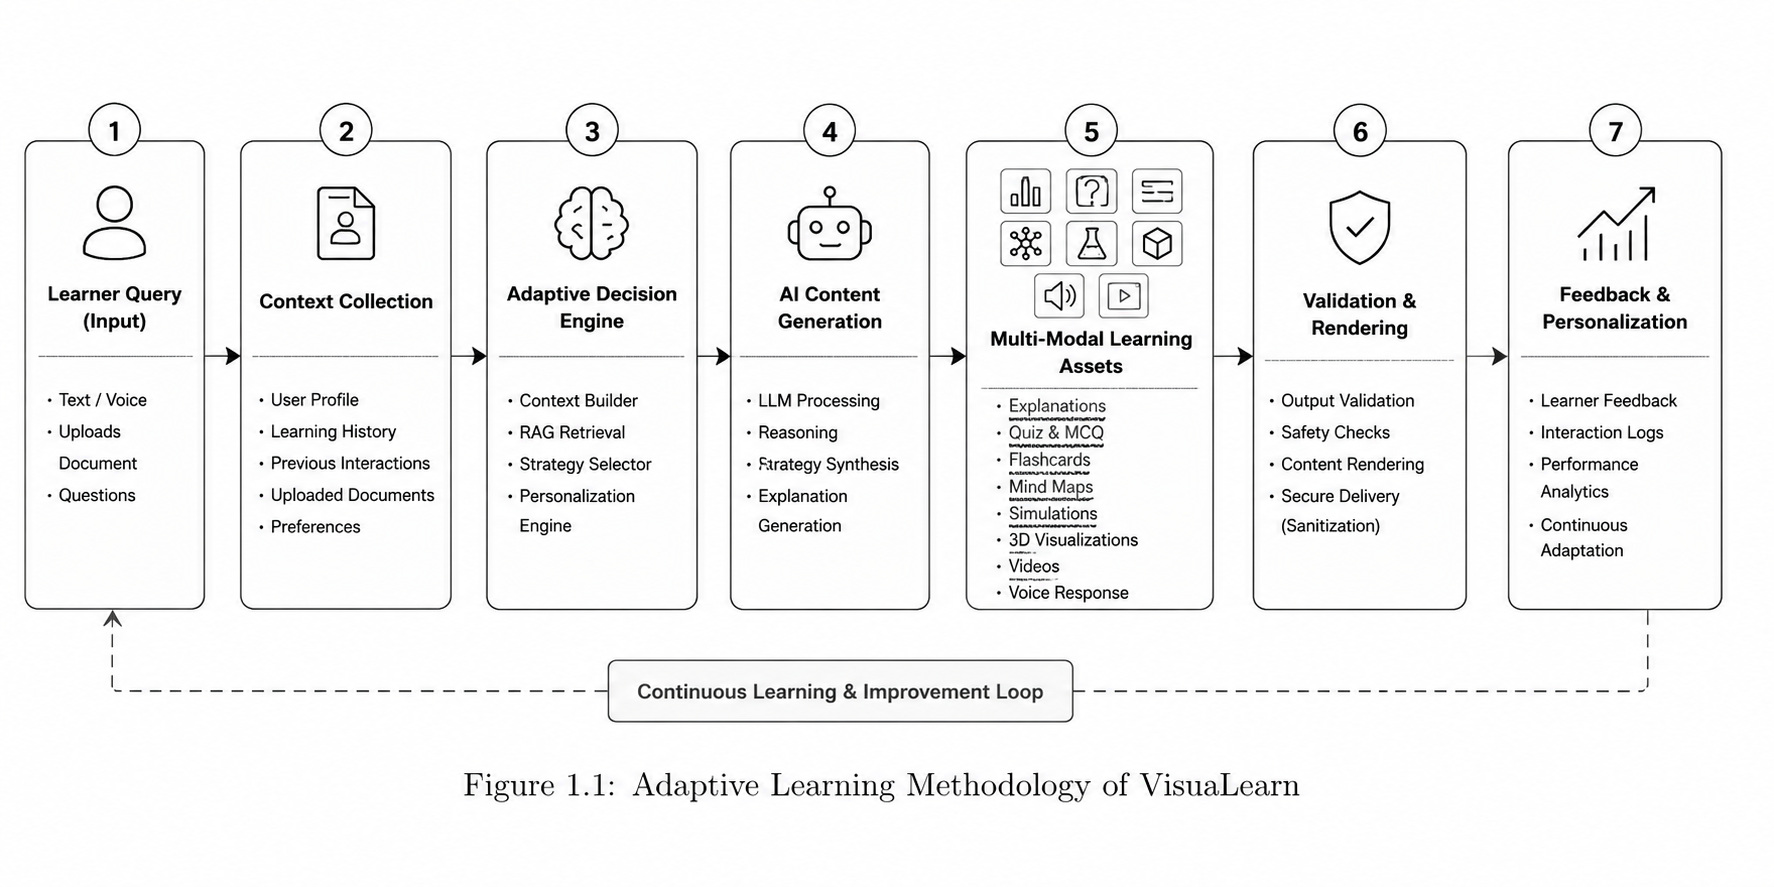
\includegraphics[width=0.95\textwidth]{Chapter1/1.1}
\caption{High-level methodology and adaptive learning workflow}
\label{fig:methodology}
\end{figure}

\section[Assumptions made / Constraints of the project]{\textbf{Assumptions made / Constraints of the project}}

The project assumes that users have internet access, a modern browser, and a valid Supabase login. The backend requires configured environment variables for Supabase and AI-provider services. Optional features such as text-to-speech, image generation, and real-time voice interaction depend on external provider support and browser permissions.

The main constraints are API cost, model latency, external service availability, browser performance for visual rendering, and the quality of generated learning material. The system includes validation and feedback mechanisms, but learners or teachers still need to review content used for high-stakes academic work.

The implemented platform was evaluated with 30 participants using learning modules such as simulations, visual explanations, document-based learning, quizzes, and revision artifacts. The feedback from this evaluation is used in the report to discuss usability, engagement, and learner perception.
